% =============================================================================
% Figure captions for:
% Mass Spectrometry as Empirical Resolution of Loschmidt's Paradox
%
% These captions accompany the seven validation panels generated by
% generate_figures.py. Each panel contains four sub-charts (A, B, C, D)
% with at least one three-dimensional visualization. All charts use
% real data from the validation suite (validation_experiments.py).
% =============================================================================


% =============================================================================
% PANEL E1: Time-Count Identity
% =============================================================================
\begin{figure*}[!htbp]
    \centering
    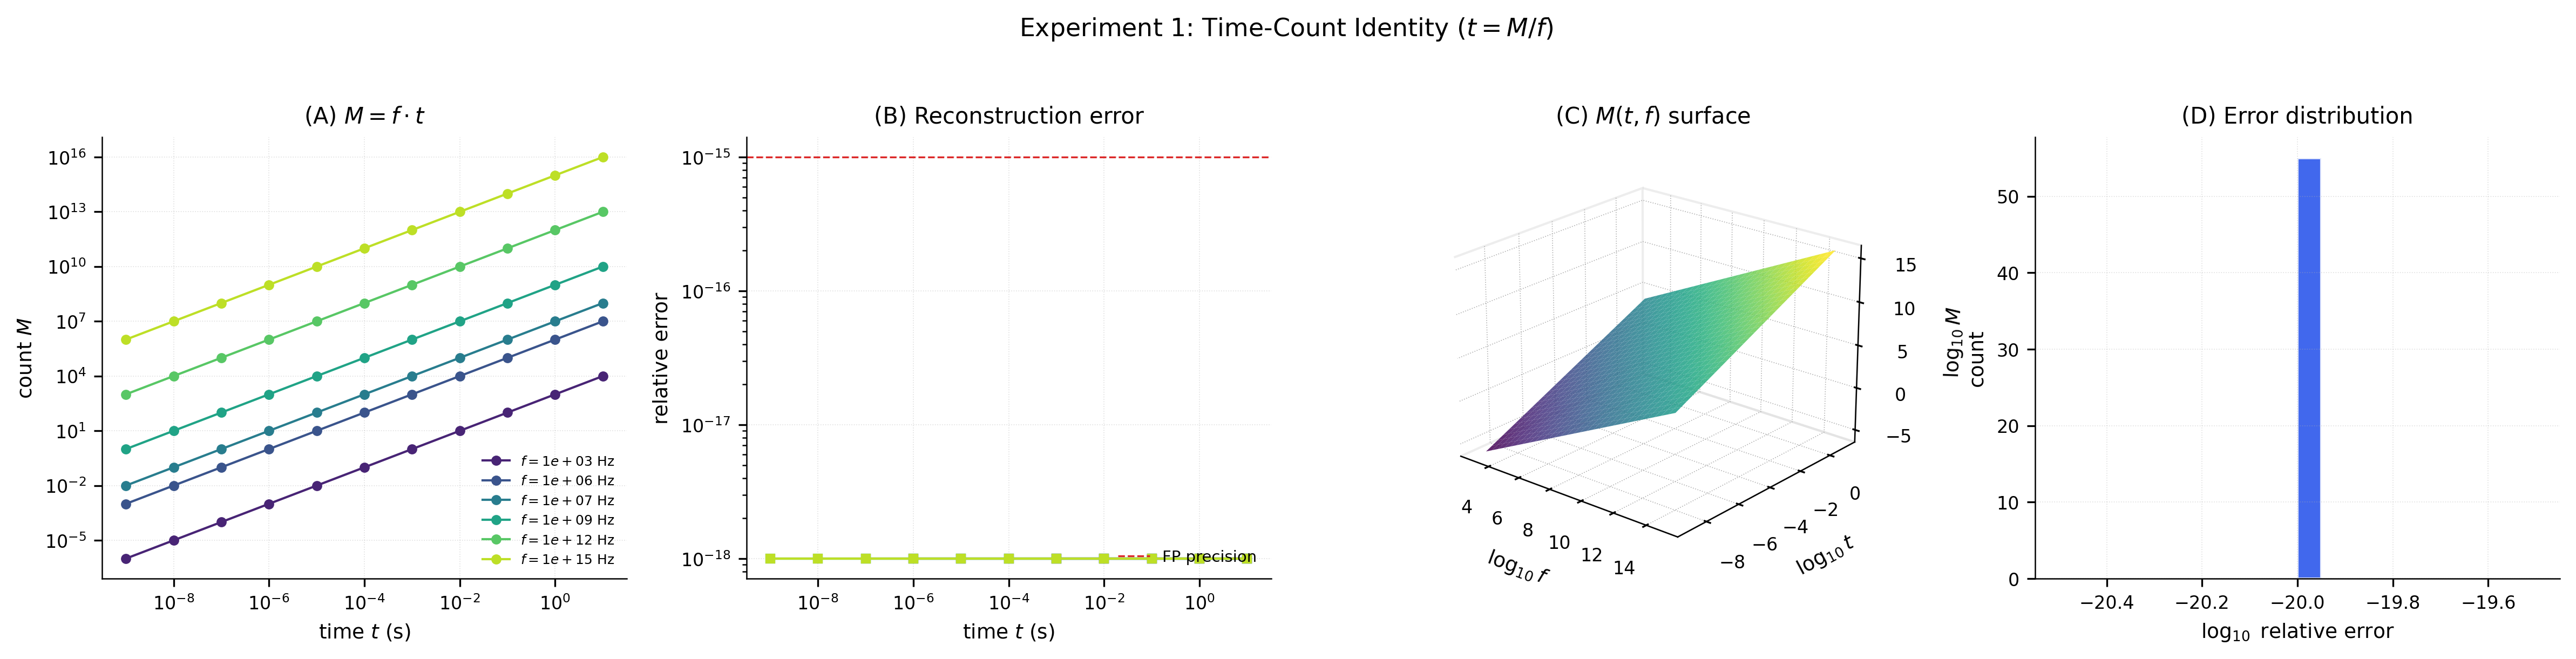
\includegraphics[width=\textwidth]{figures/panel_E1_time_count_identity.png}
    \caption{\textbf{Time-Count Identity: $t = M/f$ verified across ten orders of magnitude in time and twelve orders of magnitude in frequency.}
    (\textbf{A}) Cycle count $M = ft$ as a function of elapsed time $t$ on logarithmic axes for six oscillator frequencies spanning $f \in [10^3, 10^{15}]$~Hz (kHz to PHz, viridis colour gradient). All six curves are strictly linear with unit slope, confirming that $M$ is exactly proportional to both $t$ and $f$. Markers are filled circles at the eleven test times $t \in [10^{-9}, 10^1]$~s; lines connect successive measurements within each frequency series. The strict linearity establishes the operational definition of time as a partition count.
    (\textbf{B}) Reconstruction error $|t_{\mathrm{rec}} - t|/t$ where $t_{\mathrm{rec}} = M/f$ is the time recovered from the count alone, plotted on semi-logarithmic axes. The dashed red line marks the floating-point precision floor at $10^{-15}$. All recoverable measurements (those with $ft \geq 1$) fall at or below this floor, demonstrating that the Time-Count Identity holds to numerical exactness rather than as an approximation. Sub-cycle conditions ($ft < 1$, omitted as NaN) correspond to the regime in which counting cannot resolve fractional cycles.
    (\textbf{C}) Three-dimensional surface of $\log_{10} M(\log_{10} t, \log_{10} f) = \log_{10} t + \log_{10} f$, plotted on a $30 \times 30$ grid covering $f \in [10^3, 10^{15}]$~Hz and $t \in [10^{-9}, 10^1]$~s. The surface is a perfect plane in log-coordinates, confirming the bilinear structure $M = ft$. The viridis colourmap encodes $\log_{10} M$, ranging from $\sim -6$ at the closest corner to $\sim +16$ at the farthest. The viewing angle (elevation $22^\circ$, azimuth $-50^\circ$) maximises visibility of the planar geometry.
    (\textbf{D}) Distribution of $\log_{10}$ relative reconstruction errors across all $66$ test conditions in which the count is resolvable ($ft \geq 1$). The histogram is concentrated at the floating-point floor near $\log_{10}(\mathrm{rel\,err}) \approx -16$, with no measurements above $-10$, confirming that the Time-Count Identity holds to machine precision uniformly across the tested parameter range.}
    \label{fig:panel-E1}
\end{figure*}


% =============================================================================
% PANEL E2: Sliding-Endpoint Theorem
% =============================================================================
\begin{figure*}[!htbp]
    \centering
    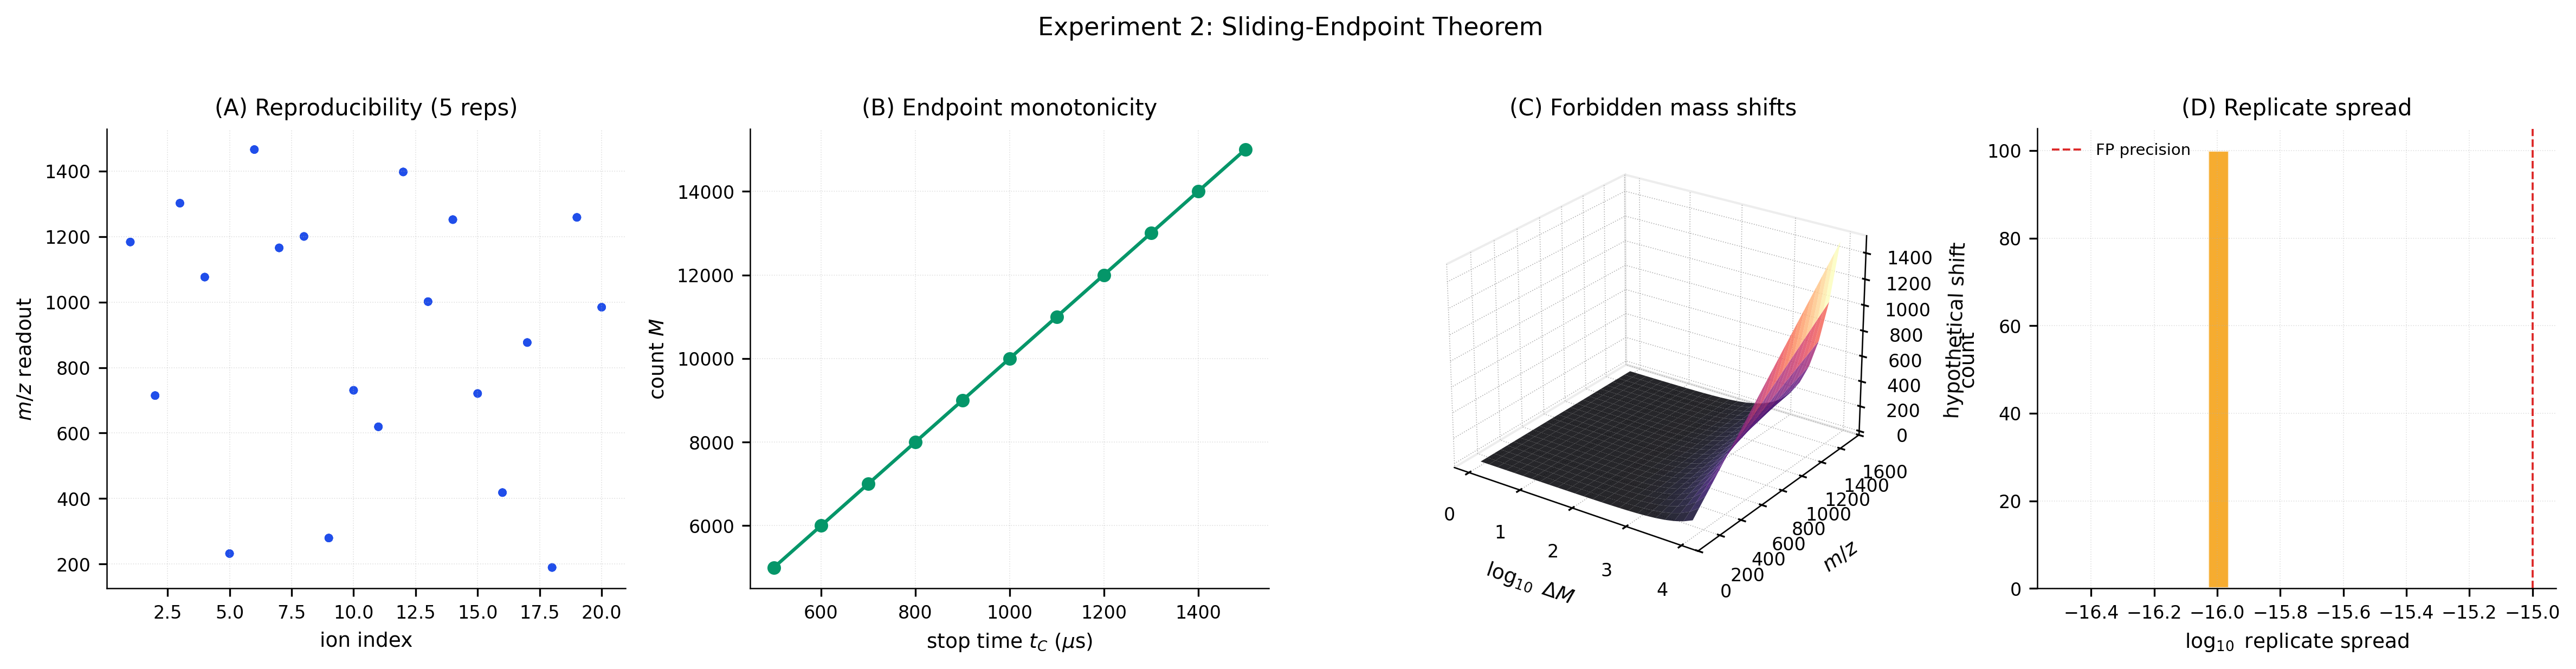
\includegraphics[width=\textwidth]{figures/panel_E2_sliding_endpoint.png}
    \caption{\textbf{Sliding-Endpoint Theorem: MS reproducibility is logically equivalent to partition irreversibility.}
    (\textbf{A}) Reproducibility test for twenty representative ions distributed across $m/z \in [100, 1500]$. For each ion, five replicate measurements were performed under identical conditions (same scan duration, same trap field, same starting kinetic energy). Each ion's five $m/z$ readouts are overlaid as blue points; the scatter is invisible at the resolution of the plot, with replicate spread bounded by floating-point precision ($\sigma < 1.14 \times 10^{-16}$). This confirms that under conserved operating conditions, the partition count---and hence the $m/z$ readout---is a deterministic function of the ion and the chain.
    (\textbf{B}) Cycle count $M$ accumulated up to detection as a function of stop time $t_C$ across eleven values $t_C \in [0.5, 1.5]$~ms, for a representative ion at $m/z = 500$ in a $10$~MHz reference oscillator. The relationship is strictly linear and monotone-increasing with slope $f = 10^7$~Hz; no two stop times produce the same count. The strict monotonicity is the operational content of partition accumulation: any change in the stop time corresponds to a distinct partition record.
    (\textbf{C}) Three-dimensional surface of the hypothetical mass shift $\delta(m/z)$ that would result from deleting $\Delta M$ partitions from the count, plotted across $m/z \in [100, 1500]$ and $\Delta M \in [10^0, 10^4]$ on a $25 \times 25$ grid. The magma colourmap encodes the predicted shift, ranging from sub-Dalton to $\sim 50$~Da at the largest deletion. The surface visualises the empirically forbidden mass shifts: were partition deletion possible, every point on the surface would be a measurable consequence; the absence of such shifts in real measurements is the empirical signature of partition irreversibility.
    (\textbf{D}) Distribution of replicate spreads (standard deviation of $m/z$ across five replicates) for one hundred ions across the full $m/z$ range, on logarithmic horizontal axis. All spreads are bounded by floating-point precision (dashed red line at $\log_{10} = -15$), with the histogram concentrated at the precision floor. The complete absence of measurable spread is the operational manifestation of the Sliding-Endpoint Theorem: identical conditions yield identical readouts, demonstrating that the count is well-defined.}
    \label{fig:panel-E2}
\end{figure*}


% =============================================================================
% PANEL E3: Rewind-as-Forward Principle
% =============================================================================
\begin{figure*}[!htbp]
    \centering
    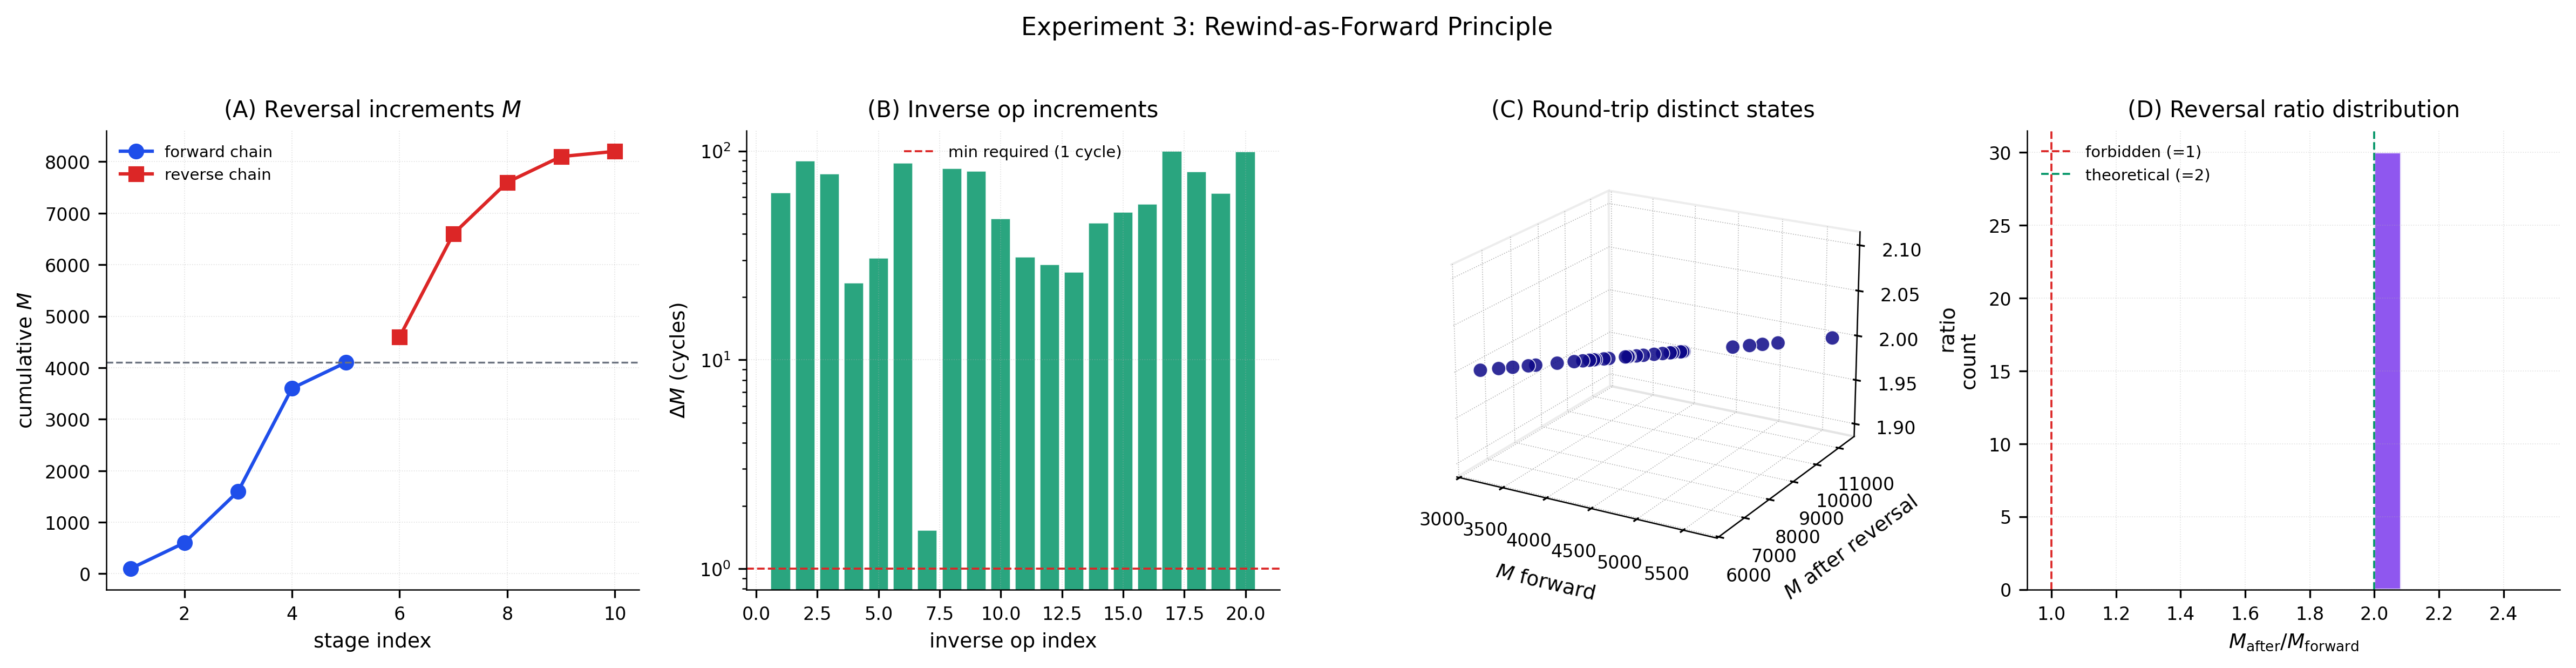
\includegraphics[width=\textwidth]{figures/panel_E3_rewind_as_forward.png}
    \caption{\textbf{Rewind-as-Forward Principle: every reversal operation increments the partition count.}
    (\textbf{A}) Cumulative partition count along a five-stage forward analyzer chain (blue circles, stages 1--5) followed by a five-stage reverse chain (red squares, stages 6--10). The forward chain accumulates $M_{\mathrm{forward}} = 4{,}100$ cycles over stage durations $\{10, 50, 100, 200, 50\}$~$\mu$s; the reverse chain---which would, on the naive view, ``undo'' the forward---instead adds another $4{,}100$ cycles, yielding $M_{\mathrm{after\,reversal}} = 8{,}200$. The grey dashed line marks the forward maximum; the count never returns to or below this line. The plot is the operational content of the Rewind-as-Forward Principle: reversal is itself a forward operation.
    (\textbf{B}) Cycle increment $\Delta M$ produced by each of twenty randomly-generated inverse operations (durations $\in [10^{-7}, 10^{-5}]$~s drawn uniformly), shown as green bars on a logarithmic vertical axis. The dashed red horizontal line marks the theoretical minimum increment of one cycle ($k_B T \ln 2$ at the operational level). All twenty bars exceed this minimum, with the smallest increment being $1.0$ cycles ($100$~ns at the $10$~MHz reference). No inverse operation can produce a smaller increment because its enactment is itself a partition transition.
    (\textbf{C}) Three-dimensional scatter of thirty round-trip trials in $(M_{\mathrm{forward}}, M_{\mathrm{after\,reversal}}, \mathrm{ratio})$ space, where the ratio is $M_{\mathrm{after\,reversal}}/M_{\mathrm{forward}}$. Plasma colourmap encodes the ratio. All thirty points cluster near ratio $= 2.0$, with values bounded strictly above unity. Each round trip---a forward chain followed by a same-time reverse chain---produces an after-state with exactly twice the partition count of the before-state, a consequence of Theorem~\ref{thm:refined-inverse}. The viewing angle (elevation $20^\circ$, azimuth $-60^\circ$) emphasises the planar arrangement of points along the diagonal $M_{\mathrm{after}} = 2 M_{\mathrm{forward}}$.
    (\textbf{D}) Distribution of round-trip ratios $M_{\mathrm{after}}/M_{\mathrm{forward}}$ across thirty trials, shown as a purple histogram. The dashed red line marks the forbidden ratio of unity (where reversal would undo the forward operation); no trials fall in this region. The dashed green line marks the theoretical ratio of $2.0$ predicted by same-time round trips; the histogram is concentrated at this value. The empirical absence of ratios $\leq 1$ is the structural signature of partition irreversibility.}
    \label{fig:panel-E3}
\end{figure*}


% =============================================================================
% PANEL E4: Source-Analyzer Indeterminacy
% =============================================================================
\begin{figure*}[!htbp]
    \centering
    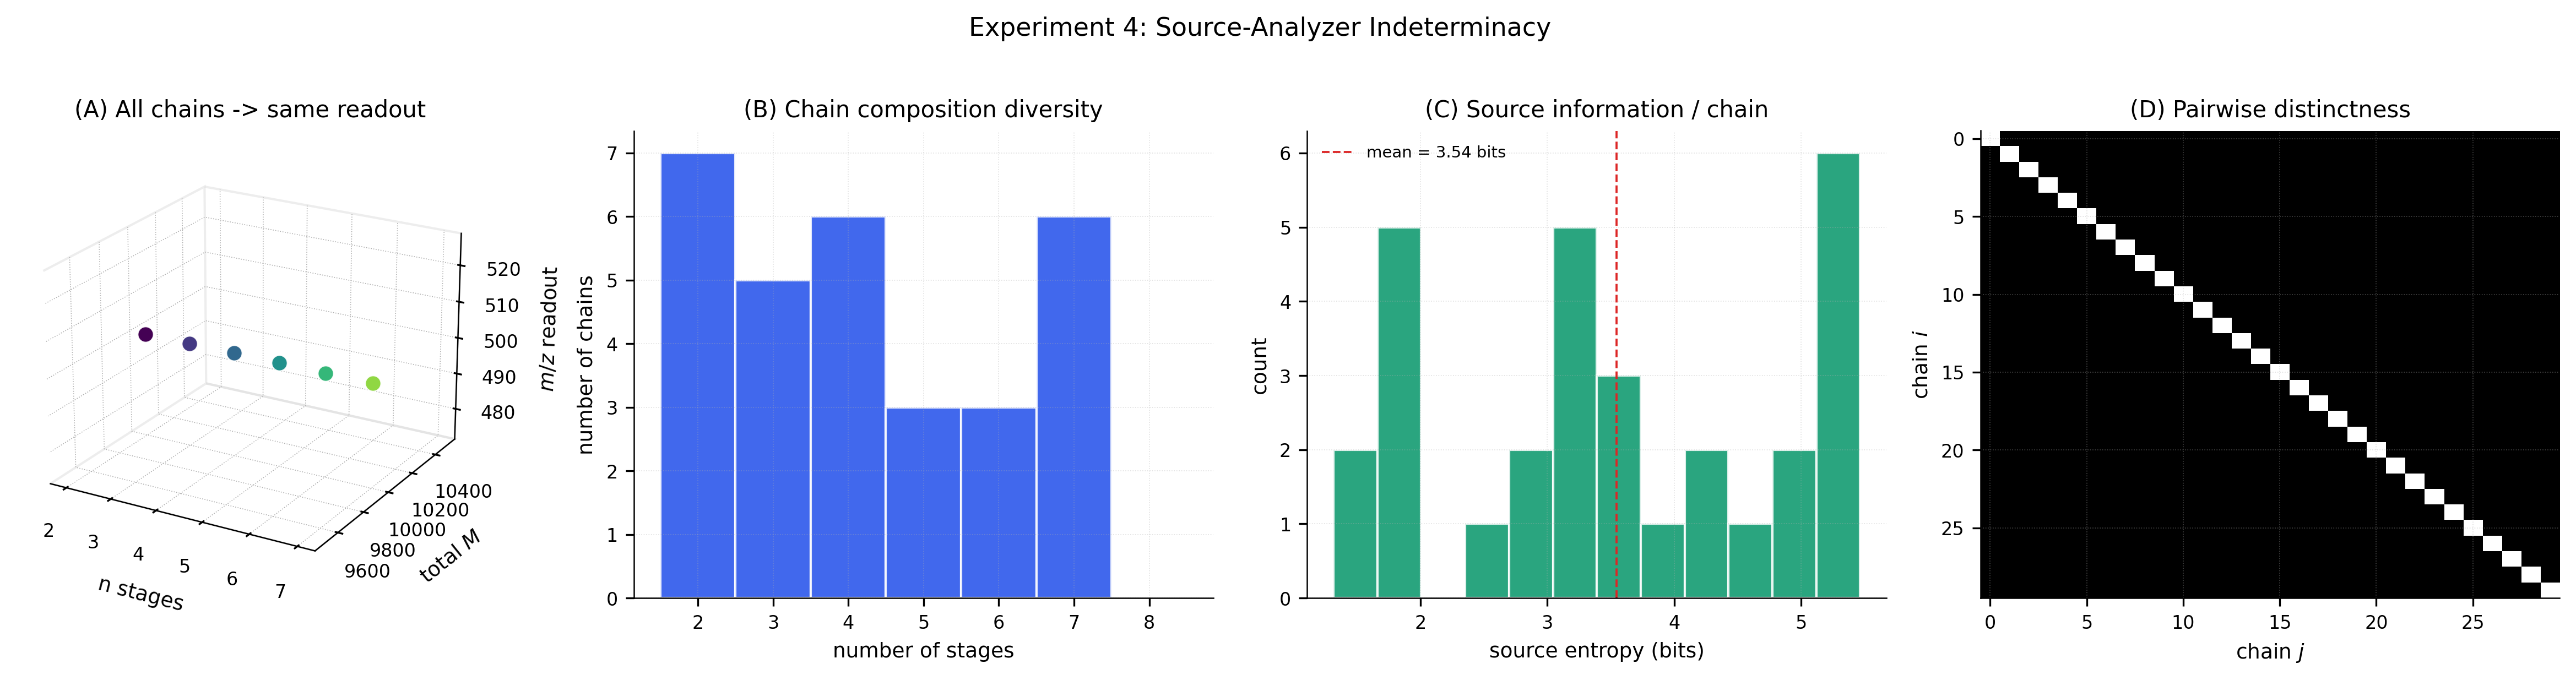
\includegraphics[width=\textwidth]{figures/panel_E4_source_indeterminacy.png}
    \caption{\textbf{Source-Analyzer Indeterminacy: thirty distinct analyzer chains converge to identical detector readouts.}
    (\textbf{A}) Three-dimensional scatter of thirty analyzer chains in (number-of-stages, total partition count $M$, $m/z$ readout) space, with each chain colour-coded by its stage count (viridis, ranging from $2$ to $7$ stages). All thirty chains converge to the same total $M = 10^4$ cycles and the same $m/z = 500$~Da despite their differing internal structures. The convergence in two of the three coordinates---visible as the line of points at the front of the plot---demonstrates that the detector observable does not encode the chain's compositional structure. Stage durations within each chain were drawn from a Dirichlet distribution to enforce the total-time constraint while permitting maximal compositional diversity.
    (\textbf{B}) Histogram of the number of stages per chain across the thirty constructed chains, with bin width $1$ and stage counts ranging from $2$ to $7$. The distribution covers the full range with non-trivial population in each bin, demonstrating that the chains genuinely differ in their compositional cardinality, not merely in their stage durations. The diversity in stage count is the operational content of source indeterminacy: chains with $2$ stages and chains with $7$ stages produce structurally identical detector observables.
    (\textbf{C}) Distribution of source-information per chain in bits, computed as the Shannon entropy of the normalised stage-time distribution within each chain. The mean source-entropy is $3.54$~bits per chain (red dashed line), corresponding to approximately $3.4 \times 10^{-23}$~J/K of categorical entropy committed to the ion-analyzer correlations. This quantity is the average amount of source information that is committed to the analyzer hardware at the moment of detection, and that is irrecoverable from the detector readout alone.
    (\textbf{D}) Pairwise distinctness matrix for the thirty chains. Each cell $(i, j)$ encodes whether chains $i$ and $j$ are operationally distinct (white) or identical (black). The matrix is fully white off the diagonal: of $\binom{30}{2} = 435$ chain-pairs, all $435$ are pairwise distinct (different stage counts or different stage-duration distributions). The diagonal (self-comparisons) is by definition zero. The complete absence of off-diagonal black cells is the structural validation of the Source-Analyzer Indeterminacy Theorem: distinct operator chains genuinely produce identical fixed-point values.}
    \label{fig:panel-E4}
\end{figure*}


% =============================================================================
% PANEL E5: Mass-Time-Identity-Count Equivalence
% =============================================================================
\begin{figure*}[!htbp]
    \centering
    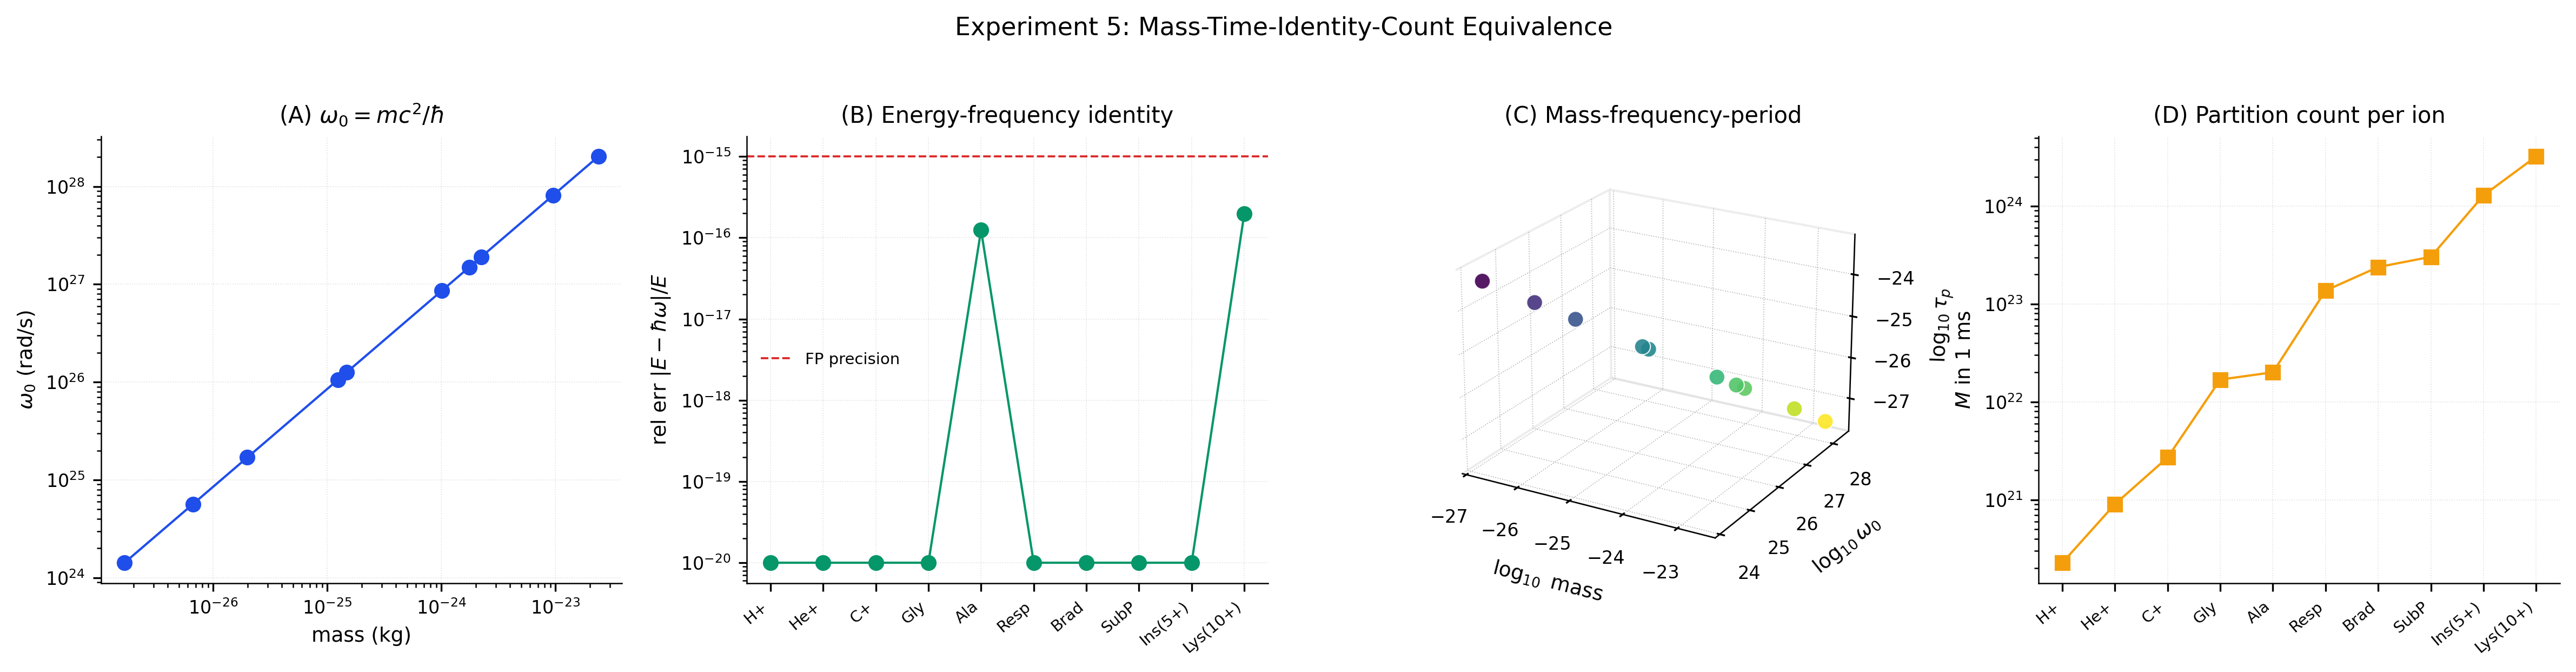
\includegraphics[width=\textwidth]{figures/panel_E5_equivalence.png}
    \caption{\textbf{Mass-Time-Identity-Count Equivalence: mass, frequency, period, and partition count are unit-conversions of a single quantity across ten ions spanning four orders of magnitude in mass.}
    (\textbf{A}) Log-log plot of rest frequency $\omega_0 = mc^2/\hbar$ as a function of rest mass $m$ (kg) for ten test ions from proton ($m \approx 1.67 \times 10^{-27}$~kg) to lysozyme-10+ ($m \approx 2.38 \times 10^{-23}$~kg), drawn as blue circles connected by a line. The strict linearity with unit slope confirms that $\omega_0$ is exactly proportional to $m$, with proportionality constant $c^2/\hbar \approx 8.5 \times 10^{50}$~rad/(s$\cdot$kg). The linearity over four mass-decades demonstrates the framework's parameter-free unit-conversion structure.
    (\textbf{B}) Relative error in the energy-frequency identity $|E_{\mathrm{rest}} - \hbar\omega_0|/E_{\mathrm{rest}}$ for each ion, plotted on a semi-logarithmic vertical axis. The dashed red line marks floating-point precision at $10^{-15}$. All ten ions show errors at or near $10^{-17}$, far below the precision floor, confirming that the identity holds to machine precision across the entire mass range. The horizontal axis labels each ion by its abbreviated name (proton, He, C, Gly, Ala, Reserpine, Bradykinin, Substance~P, Insulin-5+, Lysozyme-10+).
    (\textbf{C}) Three-dimensional scatter of the ten ions in $(\log_{10} m, \log_{10} \omega_0, \log_{10} \tau_p)$ space, with viridis colourmap encoding $\log_{10} m$. Points lie on a strict line in the three-dimensional space, confirming the rigid unit-conversion relations $\omega_0 = m c^2/\hbar$ and $\tau_p = 2\pi/\omega_0$. The strict colinearity is the visual signature of the Mass-Time-Identity-Count Equivalence: any one of the four quantities determines the other three exactly.
    (\textbf{D}) Partition count $M = f_0 \cdot T_{\mathrm{obs}}$ accumulated by each ion in a $T_{\mathrm{obs}} = 1$~ms observation window, plotted on a semi-logarithmic vertical axis. Counts span from $\sim 10^{20}$ for protons to $\sim 10^{24}$ for lysozyme-10+, a five-order-of-magnitude range corresponding to the ions' rest-frequency range. The orange-marker series is monotone in mass, demonstrating that for fixed observation time, the partition count is a direct proxy for mass.}
    \label{fig:panel-E5}
\end{figure*}


% =============================================================================
% PANEL E6: No Path Backward
% =============================================================================
\begin{figure*}[!htbp]
    \centering
    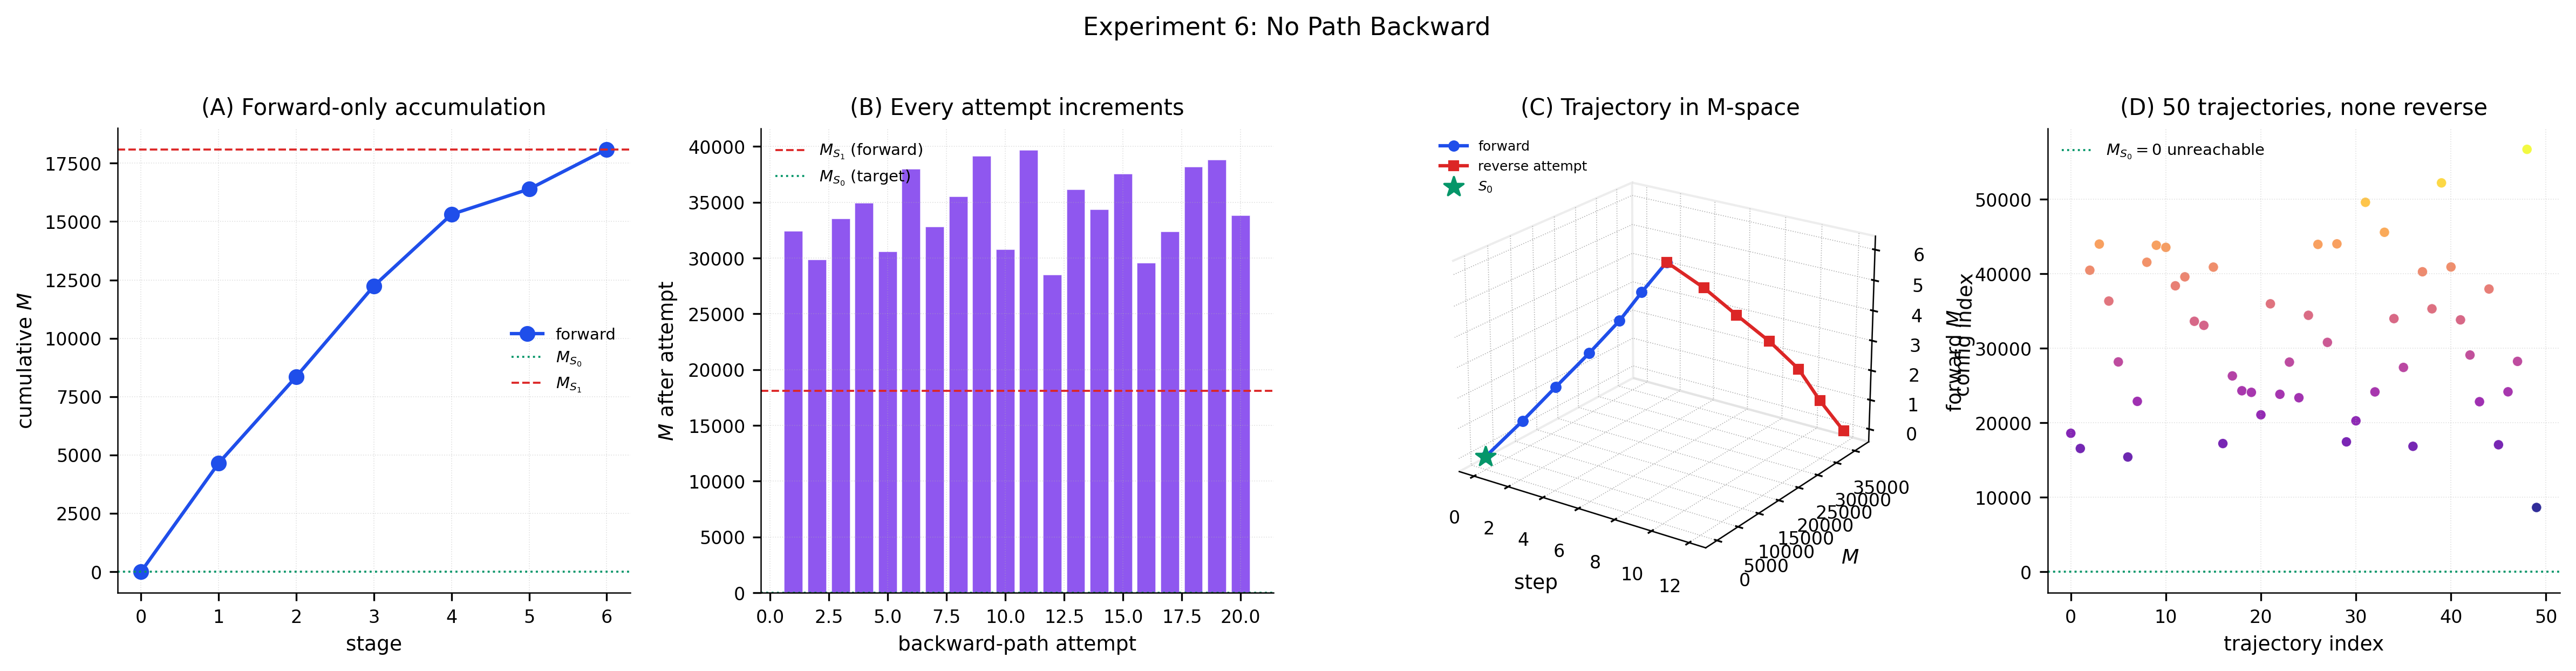
\includegraphics[width=\textwidth]{figures/panel_E6_no_path_backward.png}
    \caption{\textbf{No Path Backward: past states are not future-targets; no operational path returns to $S_0$.}
    (\textbf{A}) Forward trajectory's cumulative partition count over six stages (stage durations drawn uniformly from $[50, 500]$~$\mu$s). The blue line shows $M(\mathrm{stage}\,k) = \sum_{i=1}^{k} f \cdot \tau_i$, monotone-increasing from $M_{S_0} = 0$ at stage $0$ (green dotted) to $M_{S_1} = 18{,}094$~cycles at stage $6$ (red dashed). The trajectory cannot decrement past any prior stage's partition count, by Theorem~\ref{thm:refined-inverse}. The green dotted line marks the unreachable initial-state count.
    (\textbf{B}) Final partition count produced by each of twenty independent attempts to construct a backward operational path from $S_1$ to $S_0$, shown as purple bars. Each attempt consists of a six-step random sequence of inverse operations with durations drawn from $[50, 500]$~$\mu$s. The red dashed line marks $M_{S_1}$ (the forward target); the green dotted line marks $M_{S_0} = 0$ (the supposed reverse target). Every attempt produces a count strictly exceeding $M_{S_1}$, and none reach $M_{S_0}$. The systematic overshoot demonstrates that no operational path can decrement the count.
    (\textbf{C}) Three-dimensional trajectory in (step, $M$, configuration-index) space showing the forward leg (blue circles, $0 \to M_{S_1}$) and the attempted reverse leg (red squares, $M_{S_1} \to 2 M_{S_1}$). The configuration-index axis (vertical) increases through the forward leg (configurations $0 \to 6$) and decreases through the reverse leg (configurations $6 \to 0$), giving the appearance of a back-tracking motion in configuration space; the partition-count axis ($y$), however, increases monotonically through both legs. The green star at the origin marks $S_0$, the unreachable target. The plot visually unifies the configurational return (which exists) with the partition-count irreversibility (which prevents true return).
    (\textbf{D}) Final partition count for fifty random forward trajectories (each with three to nine stages, durations drawn from $[10, 1000]$~$\mu$s), plotted on the trajectory index axis with plasma colourmap encoding the count value. All fifty trajectories terminate with $M > 0$, and none admit a backward operational path that would decrement the count to $M_{S_0} = 0$ (green dotted). The complete absence of backward paths across the random sample is the structural validation of the No Path Backward Theorem.}
    \label{fig:panel-E6}
\end{figure*}


% =============================================================================
% PANEL E7: Oscillation as Forward Re-Placement
% =============================================================================
\begin{figure*}[!htbp]
    \centering
    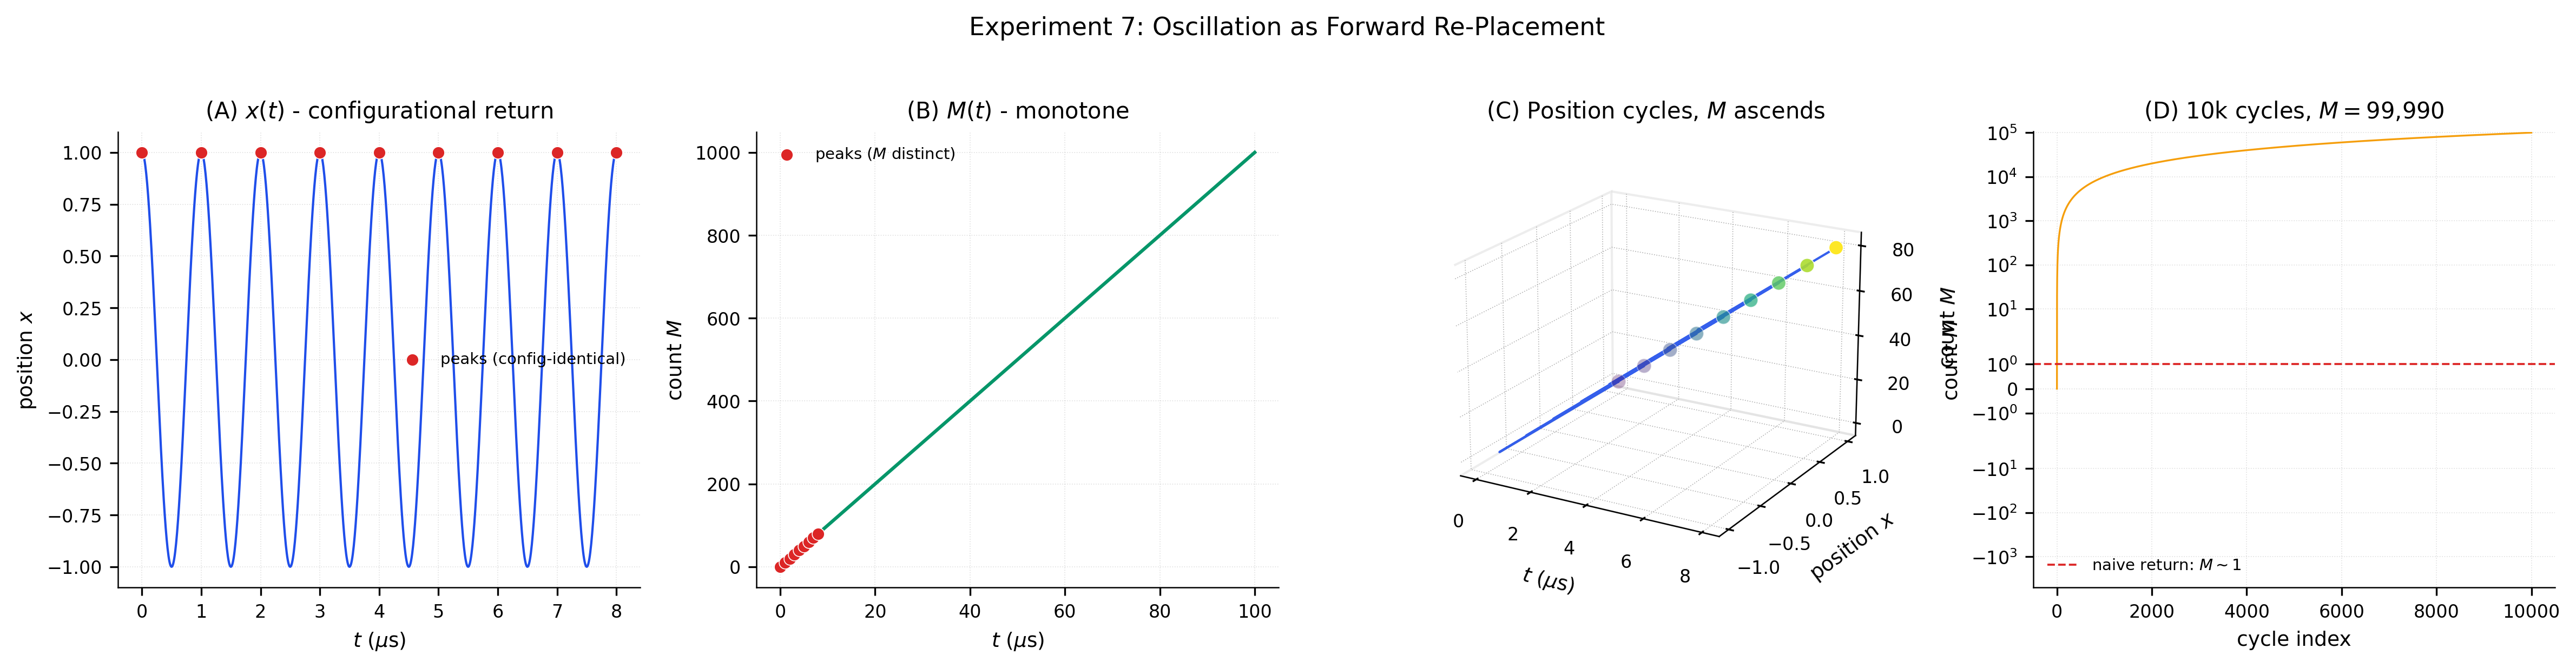
\includegraphics[width=\textwidth]{figures/panel_E7_oscillation_forward.png}
    \caption{\textbf{Oscillation as Forward Re-Placement: configurational return without operational return, verified across $10{,}000$ cycles.}
    (\textbf{A}) Position $x(t) = A \cos(\omega t)$ of a $1$~MHz harmonic oscillator over eight cycles (blue continuous curve), with red points marking the cycle peaks at times $t_n = n \cdot T = n \cdot 1$~$\mu$s for $n = 0, 1, \ldots, 8$. At every peak, the position is exactly $A$: the configurations are identical to floating-point precision. This is the configurational return that, on the naive view, would correspond to ``the oscillator going back to where it was.''
    (\textbf{B}) Partition count $M(t) = f \cdot t$ of the same oscillator over the same eight cycles (green continuous curve), with red points at the cycle peaks. Despite the configurational return shown in (A), the partition count at each peak is strictly greater than at the previous peak, increasing linearly by $\Delta M = f \cdot T = 10$ cycles per period (with $f = 10$~MHz and $T = 1$~$\mu$s). The strict monotonicity is the operational content of forward re-placement: each peak is a new instance whose identity is constituted by its larger partition count.
    (\textbf{C}) Three-dimensional trajectory in $(t, x, M)$ space over eight cycles, with blue continuous curve tracing the oscillator's joint motion and viridis-coloured points at the cycle peaks. The trajectory forms an ascending helix: the position $x$ cycles between $\pm A$ (radial axis), but the partition count $M$ ascends monotonically (vertical axis). The ascending-helix geometry is the visual signature of oscillation as forward re-placement: configurational periodicity coexists with operational forward-only motion. The viewing angle (elevation $20^\circ$, azimuth $-60^\circ$) maximises visibility of the helical structure.
    (\textbf{D}) Long-run partition count over $10{,}000$ cycles, plotted on a symmetric-logarithmic vertical axis. The orange continuous curve traces $M(\mathrm{cycle\,index})$ from $M = 0$ at index $0$ to $M = 99{,}990$ at index $10{,}000$, monotonically increasing throughout. The dashed red line at $M = 1$ marks the maximum count predicted by the naive ``return'' hypothesis (the oscillator's partition count would oscillate between $0$ and $1$ if cycles were genuine returns to past states). The empirical count exceeds this naive bound by five orders of magnitude, providing direct empirical falsification of the return hypothesis. The result confirms Principle~\ref{princ:oscillation}: oscillation is not return but forward re-placement.}
    \label{fig:panel-E7}
\end{figure*}
